\documentclass[11pt,a4paper]{article}

\usepackage[T1]{fontenc}
\usepackage[utf8]{inputenc}
\usepackage[italian]{babel}
\usepackage{amsmath,amssymb}
\usepackage[a4paper,margin=2.5cm]{geometry}
\usepackage{array}
\usepackage{siunitx}
\usepackage{booktabs}
\usepackage{graphicx}
\usepackage{float}
\usepackage{hyperref}

\hypersetup{hidelinks}
\setlength{\parindent}{0pt}
\setlength{\parskip}{4pt}
\allowdisplaybreaks
\graphicspath{{figure/}}
\sisetup{output-decimal-marker={,}, group-separator={\,}, per-mode=symbol,
         exponent-product=\cdot, range-phrase={\text{--}}}

\newcommand{\uma}{u-a}
\newcommand{\upa}{u+a}
\newcommand{\Ms}{M_{s}}

\title{Gasdinamica -- Svolgimento esercizio 2\\[2pt]
\large Pistone con legge parabolica e poi lineare: formazione dell'urto, transitorio e regime asintotico}
\author{}
\date{Prova del 01/02/1970}

\begin{document}
\maketitle

\section*{Traccia}
Un pistone posto all'estremo sinistro di un condotto molto lungo si muove verso destra con legge parabolica
$x=t^2$ fino a $t=1$ e, dopo tale istante, con legge lineare $x=2t-1$. Il gas nel condotto è in quiete con
pressione $p=1$ e densità $\rho=\gamma$. Determinare l'evoluzione del campo e la sua dipendenza dal peso
molecolare del gas (proprietà $\gamma$ e $R$). Descrivere il campo nei piani spazio--tempo e pressione--velocità.
\begin{figure}[H]
  \centering
  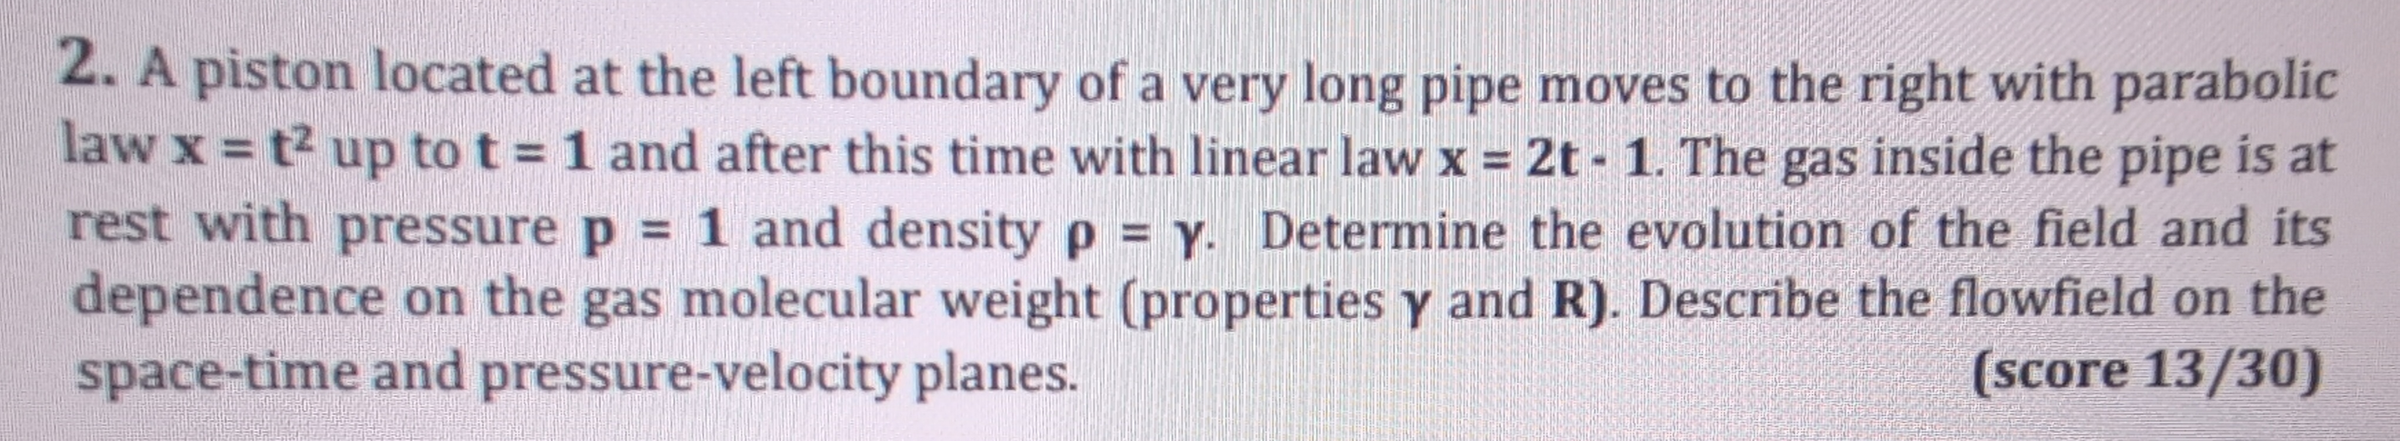
\includegraphics[width=0.85\textwidth]{originale.png}
  \caption{Testo originale dell'esercizio.}
\end{figure}
La traccia coincide con l'esercizio 2 della prova del 25/01/2023 (B69-E02 del catalogo); tracce dello stesso tipo
(pistone accelerato e poi a velocità costante) sono B49-E01 e B20-E01.

%==============================================================================
\section{Lettura del testo e dati}
La legge del pistone dà
\[
x_p=t^2,\quad u_p=2t,\quad \ddot x_p=2\quad(0\le t\le1);\qquad x_p=2t-1,\quad u_p=2,\quad \ddot x_p=0\quad(t>1).
\]
Posizione e velocità sono continue in $t=1$; è discontinua solo l'accelerazione. Anche in $t=0$ la velocità è
continua ($u_p(0)=0$), mentre l'accelerazione passa da 0 a 2.

Il dato $\rho=\gamma$ con $p=1$ non è casuale: la velocità del suono del gas indisturbato è
\[
a_0=\sqrt{\gamma p_0/\rho_0}=1
\]
\textbf{per qualunque gas}. Tutte le velocità sono quindi riferite ad $a_0$ e il pistone raggiunge
$u_p=2a_0$. La temperatura iniziale invece dipende dal gas, $T_0=p_0/(\rho_0R)=1/(\gamma R)$.

\begin{table}[H]
  \centering
  \begin{tabular}{lll}
    \toprule
    Grandezza & Valore & Note \\
    \midrule
    $p_0$, $\rho_0$, $u_0$ & $1$, $\gamma$, $0$ & stato 0, gas in quiete \\
    $a_0$ & $1$ & per ogni $\gamma$ \\
    $T_0$ & $1/(\gamma R)$ & dipende da $R$ \\
    $u_p$ & $2t$ per $t\le1$, $2$ per $t>1$ & pistone a sinistra \\
    $\gamma$ & \num{1.4} (aria) per i valori numerici & confronto con elio ($\gamma=5/3$) e SF$_6$ ($\gamma\approx\num{1.1}$) \\
    \bottomrule
  \end{tabular}
  \caption{Dati del problema.}
\end{table}
Interpretazione: la traccia non fissa il gas e chiede la dipendenza da $\gamma$ ed $R$. Svolgo il problema in forma
letterale in $\gamma$, do i valori numerici per l'aria e li confronto con un gas leggero monoatomico (elio) e con
un gas pesante poliatomico (SF$_6$).

%==============================================================================
\section{Modello e ipotesi}
\begin{itemize}
\item \textbf{Eulero 1D instazionario}, gas perfetto, non viscoso e adiabatico: il condotto è a sezione costante e
  molto lungo, quindi le onde sono piane e l'estremo destro non interviene (nessuna riflessione).
\item \textbf{Onda semplice omoentropica} finché non si forma l'urto: lo stato iniziale è uniforme e in quiete,
  e il pistone, partendo con velocità nulla, genera onde di una sola famiglia.
\item Dopo la formazione dell'urto il flusso non è più omoentropico. Per gli stati dopo che l'urto ha assorbito
  l'intera compressione uso un \textbf{pseudo-problema di Riemann} fra gli stati esterni, che dà gli stati medi ma
  non la struttura interna della zona d'interazione. Il regime asintotico lo ottengo con il pistone a velocità
  costante.
\item Gli istanti d'incontro dopo la formazione li stimo con caratteristiche rettilinee anche nelle zone
  d'interazione.
\end{itemize}

%==============================================================================
\section{Analisi qualitativa}
Il pistone è a sinistra del gas e avanza: genera una \textbf{compressione della famiglia $\upa$}, che spinge il gas
verso destra, nel verso in cui si propaga. Poiché $u_p(0)=0$, in $(0,0)$ non c'è alcuna singolarità: la testa
della compressione è la caratteristica $x=a_0t$ e su di essa è discontinuo solo il gradiente. La compressione è
\textbf{non centrata}: si forma per accelerazione continua del pistone.

In un'onda semplice $\upa$ ogni caratteristica è una retta e trasporta lo stato del pistone all'istante di
emissione. Le caratteristiche emesse più tardi hanno $u$ e $a$ maggiori, quindi sono più veloci e raggiungono
quelle emesse prima: la compressione si irripidisce e, per \textbf{coalescenza}, degenera in un urto
(``la compressione degenera''). L'urto nasce di intensità nulla nel punto di blow-up e poi si rinforza assorbendo
le caratteristiche che lo raggiungono da sinistra.

Dopo $t=1$ il pistone ha velocità costante: l'ultima caratteristica di compressione parte da $(1,1)$ e fra essa e
il pistone c'è un plateau uniforme 1. Il gas è stato compresso isentropicamente, mentre l'urto, a parità di
velocità del gas, dà una pressione minore: la curva di Rankine--Hugoniot sta sotto l'isentropica. Quando l'urto
ha assorbito tutta la compressione, il disaccordo fra lo stato 1 e lo stato che l'urto può sostenere si risolve,
come al centro di una compressione centrata, con un \textbf{urto $\upa$, un contatto e un'espansione $\uma$}
(configurazione RCS). L'espansione $\uma$ torna verso il pistone e si riflette con la stessa natura (espansione
$\upa$), insegue l'urto e lo indebolisce. A tempi lunghi resta il campo del pistone impulsivo a velocità $2$, con in
più la memoria del transitorio: uno strato entropico.

%==============================================================================
\section{Topologia del campo}
\begin{table}[H]
  \centering
  \small
  \begin{tabular}{clp{8.2cm}}
    \toprule
    Stato & Dove & Onda che lo separa dagli stati vicini \\
    \midrule
    0 & gas indisturbato & a destra della testa $x=t$ (poi dell'urto) \\
    -- & onda semplice $\upa$ & caratteristiche rettilinee emesse per $0\le t_p\le1$ \\
    1 & plateau, $u=2$ & fra il pistone ($t>1$) e la coda della compressione, uscente da $(1,1)$ \\
    2, 3 & dietro l'urto, dopo A & pseudo-Riemann 1|0: espansione $\uma$ (1--2), contatto (2--3), urto $\upa$ (3--0) \\
    4 & sul pistone & riflessione dell'espansione $\uma$: espansione $\upa$ \\
    5, 6 & regime asintotico & gas mai urtato sul pistone (5), contatto/strato entropico, gas urtato (6), urto \\
    \bottomrule
  \end{tabular}
  \caption{Stati e onde. A è il punto in cui l'urto raggiunge la coda della compressione.}
\end{table}
Nel piano $x$--$t$ ci sono una zona a 0 famiglie (stato 0, e poi i plateau 1 e 4), una zona a 1 famiglia (l'onda
semplice fra il pistone e l'urto, con le caratteristiche $\upa$ semirette) e, dopo A, zone d'interazione a due
famiglie vicino al pistone (espansione $\uma$ e sua riflessa) e dove l'espansione riflessa attraversa il contatto
e raggiunge l'urto. I contorni fra 0 e l'onda semplice (la testa $x=t$) e fra l'onda semplice e il plateau 1 (la
coda) sono semirette, finché l'urto non le raggiunge.

%==============================================================================
\section{Scorciatoie fisiche}
\begin{itemize}
\item In tutta l'onda semplice $\upa$ l'invariante dell'altra famiglia è uniforme e vale quello del gas in quiete:
  $a-\delta u=a_0=1$. Lo stato su ogni caratteristica si scrive in forma chiusa, senza reticolo.
\item Lo stato 1 e lo stato 0 stanno sulla stessa isentropica $\upa$: nel pseudo-Riemann 1|0 il primo tentativo
  isentropico ridà esattamente $u^{(0)}=u_1=2$ e il residuo misura direttamente la differenza fra isentropica e
  Rankine--Hugoniot.
\item Nel regime asintotico la velocità del gas dietro l'urto è quella del pistone: l'urto è quello del pistone
  impulsivo, e la pressione segue dalla sola quantità di moto.
\end{itemize}

%==============================================================================
\section{Calcolo}

\subsection*{Onda semplice di compressione}
La caratteristica $\upa$ emessa all'istante $t_p\le1$ porta lo stato del pistone; con $a-\delta u=a_0$:
\[
u=2t_p,\qquad a=1+2\delta t_p,\qquad \lambda=u+a=1+(1+\delta)\,2t_p=1+(\gamma+1)\,t_p,
\]
\[
x=t_p^2+\left[1+(\gamma+1)t_p\right](t-t_p),\qquad
\frac{p}{p_0}=\left(\frac{a}{a_0}\right)^{\frac{2\gamma}{\gamma-1}},\qquad
\frac{\rho}{\rho_0}=\left(\frac{a}{a_0}\right)^{\frac{2}{\gamma-1}}.
\]
La testa ($t_p=0$) è $x=t$; la coda ($t_p=1$) parte da $(1,1)$ con pendenza $2+\gamma$ (aria: \num{3.4}).

\subsection*{Formazione dell'urto}
Due caratteristiche vicine si incontrano dove $\partial x/\partial t_p=0$ a $t$ fissato:
\[
2t_p+(\gamma+1)(t-t_p)-\left[1+(\gamma+1)t_p\right]=0
\ \Rightarrow\ t_{env}(t_p)=\frac{1+2\gamma t_p}{\gamma+1}.
\]
È l'inviluppo (la frontiera della soluzione a più valori). Cresce con $t_p$, quindi il primo punto di
coalescenza è sulla testa, $t_p=0$:
\[
t_{BU}=x_{BU}=\frac{1}{\gamma+1}=\frac{a_0}{(1+\delta)\,\ddot x_p(0)}\qquad(\text{aria: }t_{BU}=x_{BU}=\num{0.417}).
\]
L'urto nasce sulla testa, davanti al gas indisturbato, quando il pistone è in $x_p=t_{BU}^2=\num{0.174}$, quindi
in piena fase parabolica.

\subsection*{Stato 1: plateau a velocità del pistone}
Dalla caratteristica emessa in $t_p=1$, con $u_1=u_p=2$:
\[
a_1=a_0+\delta u_p=1+(\gamma-1)=\gamma,\qquad
p_1=\gamma^{\frac{2\gamma}{\gamma-1}},\qquad
\frac{\rho_1}{\rho_0}=\gamma^{\frac{2}{\gamma-1}},\qquad \frac{T_1}{T_0}=\gamma^2,\qquad M_1=\frac{2}{\gamma}.
\]
Aria: $a_1=\num{1.4}$, $p_1=\num{10.5}$, $\rho_1/\rho_0=\num{5.38}$, $T_1/T_0=\num{1.96}$, $M_1=\num{1.43}$.
Il plateau è supersonico: le caratteristiche $\uma$ al suo interno hanno pendenza $u_1-a_1=2-\gamma=\num{0.6}>0$,
cioè vanno verso destra nel laboratorio, ma più lentamente del pistone, che quindi le raggiunge.

\subsection*{Crescita dell'urto fino ad A}
Fra BU e A l'urto assorbe le caratteristiche dell'onda semplice a partire dalla testa. Ne stimo la traiettoria per
punti: quando l'urto raggiunge la caratteristica emessa in $t_p$, gli assegno la velocità dell'urto del problema di
Riemann fra lo stato trasportato da quella caratteristica e il gas in quiete (trascuro le onde riflesse dall'urto
stesso). La velocità cresce da $w=a_0=1$ in BU al valore del pseudo-Riemann calcolato sotto. L'urto raggiunge la
coda della compressione nel punto
\[
\text{A}:\qquad t_A\approx\num{1.34},\qquad x_A\approx\num{2.16}\qquad(\text{aria}),
\]
quando il pistone è in $x_p\approx\num{1.68}$. Lì l'urto ha assorbito tutta la compressione.

\subsection*{Stati 2 e 3: pseudo-Riemann fra 1 e 0}
In A metto a contatto lo stato 1 (sinistra) e lo stato 0 (destra). Le due curve nel piano $p$--$u$ sono
\[
u_L(p)=u_1-(p-p_1)\sqrt{\frac{A_1}{p+B_1}}\ \ (p>p_1),\qquad
u_L(p)=u_1+\frac{a_1}{\delta}\left[1-\left(\frac{p}{p_1}\right)^{\frac{\gamma-1}{2\gamma}}\right]\ \ (p\le p_1),
\]
\[
u_R(p)=u_0+(p-p_0)\sqrt{\frac{A_0}{p+B_0}}\ \ (p>p_0),\qquad A_i=\frac{2}{(\gamma+1)\rho_i},\quad
B_i=\frac{\gamma-1}{\gamma+1}p_i.
\]
\textbf{Primo tentativo isentropico.} Con
\[
z=\frac{a_0}{a_1}\left(\frac{p_1}{p_0}\right)^{\frac{\gamma-1}{2\gamma}}=1,\qquad
u^{(0)}=\frac{z(a_1+\delta u_1)-(a_0-\delta u_0)}{\delta(1+z)}=2:
\]
il tentativo isentropico restituisce lo stato 1, perché 1 e 0 stanno sulla stessa isentropica. Con $u^{(0)}=2$
l'onda sinistra è nulla, $p_2^{(0)}=p_1=\num{10.5}$, mentre l'urto destro dà $p_3^{(0)}=\num{8.73}$: a parità di $u$
l'urto sostiene una pressione minore, quindi la pressione centrale deve scendere sotto $p_1$ e $u^*$ salire sopra
$2$: a sinistra c'è un'espansione. Aggiornando $u$ finché $|p_2-p_3|$ è trascurabile:
\[
u^*=u_2=u_3=\num{2.11},\qquad p^*=p_2=p_3=\num{9.48}\qquad(\text{RCS}).
\]
Ricostruzione degli stati (espansione isentropica a sinistra, Rankine--Hugoniot a destra):
\[
a_2=a_1-\delta(u^*-u_1)=\num{1.38},\qquad \frac{\rho_2}{\rho_0}=\num{4.98},\qquad \frac{T_2}{T_0}=\num{1.90},
\]
\[
\frac{\rho_3}{\rho_0}=\frac{(\gamma+1)p^*+(\gamma-1)p_0}{(\gamma-1)p^*+(\gamma+1)p_0}=\num{3.74},\qquad
a_3=\num{1.59},\qquad \frac{T_3}{T_0}=\num{2.53}.
\]
Velocità dell'urto e fronti:
\[
w=u_0+a_0M_{rel,0},\quad
M_{rel,0}=\frac{\gamma+1}{4}\frac{u^*}{a_0}+\sqrt{1+\left(\frac{\gamma+1}{4}\frac{u^*}{a_0}\right)^2}
\ \Rightarrow\ w=\Ms=\num{2.87},
\]
espansione $\uma$ con testa $u_1-a_1=\num{0.60}$ e coda $u^*-a_2=\num{0.73}$, contatto con velocità $u^*=\num{2.11}$.

\subsection*{Stato 4: riflessione dell'espansione sul pistone}
Con caratteristiche rettilinee, la testa dell'espansione $\uma$ raggiunge il pistone in
$\text{P}:\ t\approx\num{1.69}$, $x\approx\num{2.37}$, la coda in $t\approx\num{1.72}$. Il pistone impone $u=2$,
cioè una sola condizione al contorno (una caratteristica entrante, la $\upa$); l'invariante che arriva lungo la
$\uma$ è $a-\delta u$ dello stato 2:
\[
a_4-\delta u_p=a_2-\delta u^*\ \Rightarrow\ a_4=a_2-\delta(u^*-u_p)=\num{1.36},\qquad
p_4=p_2\left(\frac{a_4}{a_2}\right)^{\frac{2\gamma}{\gamma-1}}=\num{8.50}.
\]
L'onda riflessa è un'espansione $\upa$ (sulla parete mobile l'onda si riflette con la stessa natura). La sua
testa, con pendenza $u^*+a_2=\num{3.48}$, attraversa il contatto in C ($t\approx\num{2.06}$, $x\approx\num{3.67}$)
e, con pendenza $u^*+a_3=\num{3.70}$, raggiunge l'urto in S ($t\approx\num{2.73}$, $x\approx\num{6.1}$). Da lì
l'urto rallenta.

Al contatto l'espansione passa dal gas 2 ($\rho_2a_2=\num{9.62}$) al gas 3 ($\rho_3a_3=\num{8.33}$), cioè verso
impedenza minore: oltre all'espansione trasmessa nasce una debole compressione riflessa, che torna sul pistone e
riporta la pressione da $p_4=\num{8.50}$ verso il valore asintotico \num{8.73}.

\subsection*{Stati 5 e 6: regime asintotico}
A tempi lunghi, quando tutte le onde del transitorio hanno raggiunto l'urto, il gas dietro l'urto ha la velocità del
pistone, $u_6=u_p=2$. Da massa e quantità di moto nel riferimento dell'urto,
\[
\rho_0w=\rho_6(w-u_p),\qquad p_0+\rho_0w^2=p_6+\rho_6(w-u_p)^2
\ \Rightarrow\ p_6=p_0+\rho_0\,w\,u_p,
\]
e con l'energia si ottiene l'equazione dell'urto generato da un pistone in gas fermo:
\[
w^2-(1+\delta)u_pw-a_0^2=0\ \Rightarrow\
w_\infty=\frac{(1+\delta)u_p+\sqrt{(1+\delta)^2u_p^2+4a_0^2}}{2}=\num{2.76},
\]
\[
p_6=p_5=\num{8.73},\qquad \frac{\rho_6}{\rho_0}=\frac{w_\infty}{w_\infty-u_p}=\num{3.62},\qquad
\frac{T_6}{T_0}=\num{2.41}.
\]
Il gas a contatto con il pistone (stato 5) non è mai stato urtato: ha l'entropia iniziale, $u_5=2$ e $p_5=p_6$:
\[
a_5=a_0\left(\frac{p_5}{p_0}\right)^{\frac{\gamma-1}{2\gamma}}=\num{1.36},\qquad
\frac{\rho_5}{\rho_0}=\num{4.70},\qquad \frac{T_5}{T_0}=\num{1.86}.
\]
Fra 5 e 6 c'è lo strato entropico: $p$ e $u$ uniformi, densità e temperatura variabili. Il salto d'entropia
dell'urto asintotico è $s_6/s_0=\num{1.44}$ ($\Delta s/R=\num{0.91}$), più piccolo di quello dell'urto in A,
$s_3/s_0=\num{1.50}$ ($\Delta s/R=\num{1.01}$).

\subsection*{Dipendenza dal gas}
Ripeto il calcolo per i tre gas (tab.~\ref{tab:gas} e fig.~\ref{fig:gas}). In forma letterale: $t_{BU}=1/(\gamma+1)$,
$a_1=\gamma$, $p_1=\gamma^{2\gamma/(\gamma-1)}$ e $w_\infty$ dalla formula sopra con $1+\delta=(\gamma+1)/2$
dipendono solo da $\gamma$. Per $\gamma\to1$: $t_{BU}\to1/2$, $p_1\to e^2\approx\num{7.39}$,
$w_\infty\to1+\sqrt2\approx\num{2.41}$.

La costante $R$ non compare: con i dati assegnati ($p_0$, $\rho_0$ e la legge del pistone in unità di $a_0$) le
equazioni di Eulero contengono solo $\gamma$, e $R$ entra solo nella temperatura, $T=p/(\rho R)$. I rapporti
$T/T_0$ sono quindi indipendenti da $R$; cambia la temperatura assoluta, $T_0=1/(\gamma R)$: a pari $p_0$ e
$\rho_0$ un gas pesante (piccolo $R$) è più caldo.

%==============================================================================
\section{Verifiche a posteriori}
\begin{itemize}
\item Formazione prima della fine dell'accelerazione: $t_{BU}=\num{0.417}<1$, e l'urto nasce davanti al pistone,
  $x_{BU}=\num{0.417}>x_p(t_{BU})=\num{0.174}$: verificata. Il pistone raggiungerebbe la testa $x=t$ solo in $t=1$,
  ma lì c'è già l'urto, che va più veloce della testa.
\item Primo punto di coalescenza sulla testa: $t_{env}(t_p)$ crescente con $t_p$: verificata.
\item Urto fra BU e A: velocità compresa fra quella delle caratteristiche davanti ($1$) e dietro
  ($1+(\gamma+1)t_p$) e posizione prima dell'inviluppo: verificata lungo tutta la traiettoria stimata.
\item Natura delle onde nel pseudo-Riemann: $u^*=\num{2.11}>u_1=2$ $\Rightarrow$ espansione a sinistra;
  $u^*>u_0=0$ $\Rightarrow$ urto a destra (RCS): verificata.
\item Urto: $\Ms=\num{2.87}>1$ e $s_3/s_0=\num{1.50}>1$; urto asintotico $\Ms=\num{2.76}$, $s_6/s_0=\num{1.44}>1$:
  verificata.
\item $a>0$ e $p>0$ ovunque: nascono solo compressioni ed espansioni deboli ($a_4=\num{1.36}$): verificata.
\item Condizione al pistone: una caratteristica entrante, una condizione ($u=u_p$); l'espansione riflessa ha
  $a_4<a_2$, cioè è un'espansione come previsto: verificata.
\item Validità dell'approssimazione isentropica per l'urto: con $\Ms\approx\num{2.8}$, ben oltre $\approx\num{1.2}$,
  non è lecita (lo stato 1 sovrastima la pressione del \SI{20}{\percent}): serve Rankine--Hugoniot, come fatto.
\item Regime asintotico: $p_5=p_6$, $u_5=u_6=u_p$ e $p_6-p_0=\rho_0w_\infty u_p$: verificata.
\end{itemize}

%==============================================================================
\section{Risultati}
\begin{table}[H]
  \centering
  \small
  \begin{tabular}{lll}
    \toprule
    Grandezza & Aria & \\
    \midrule
    formazione dell'urto, $t_{BU}=x_{BU}=1/(\gamma+1)$ & \num{0.417} & esatto \\
    plateau 1: $u_1=2$, $a_1=\gamma$, $p_1=\gamma^{2\gamma/(\gamma-1)}$ & $a_1=\num{1.4}$, $p_1=\num{10.5}$ & esatto \\
    punto A (urto sulla coda) & $t_A\approx\num{1.34}$, $x_A\approx\num{2.16}$ & stima \\
    pseudo-Riemann 1|0 (RCS) & $u^*=\num{2.11}$, $p^*=\num{9.48}$, $w=\num{2.87}$ & stima del modello \\
    stato 4 sul pistone & $p_4=\num{8.50}$ & stima del modello \\
    urto asintotico (pistone impulsivo) & $w_\infty=\num{2.76}$, $p_5=p_6=\num{8.73}$ & esatto \\
    stato 5 sul pistone ($s_5=s_0$) & $T_5/T_0=\num{1.86}$, $\rho_5/\rho_0=\num{4.70}$ & esatto \\
    stato 6 dietro l'urto & $T_6/T_0=\num{2.41}$, $\rho_6/\rho_0=\num{3.62}$ & esatto \\
    \bottomrule
  \end{tabular}
  \caption{Risultati per l'aria ($\gamma=\num{1.4}$).}
\end{table}

\begin{table}[H]
  \centering
  \small
  \begin{tabular}{lccc}
    \toprule
     & elio, $\gamma=5/3$ & aria, $\gamma=\num{1.4}$ & SF$_6$, $\gamma\approx\num{1.1}$ \\
    \midrule
    $t_{BU}=x_{BU}$ & \num{0.375} & \num{0.417} & \num{0.476} \\
    $p_1$; $M_1$ & \num{12.9}; \num{1.20} & \num{10.5}; \num{1.43} & \num{8.14}; \num{1.82} \\
    pseudo-Riemann: $p^*$; $u^*$; $w$ & \num{11.8}; \num{2.09}; \num{3.10} & \num{9.48}; \num{2.11}; \num{2.87} &
      \num{7.14}; \num{2.13}; \num{2.62} \\
    asintotico: $w_\infty$; $p_6$ & \num{3.00}; \num{11.0} & \num{2.76}; \num{8.73} & \num{2.50}; \num{6.50} \\
    $\rho_6/\rho_0$; $T_6/T_0$; $T_5/T_0$ & \num{3.00}; \num{3.67}; \num{2.61} & \num{3.62}; \num{2.41}; \num{1.86} &
      \num{5.00}; \num{1.30}; \num{1.19} \\
    \bottomrule
  \end{tabular}
  \caption{Dipendenza dal gas (valori asintotici esatti, pseudo-Riemann stima del modello).\label{tab:gas}}
\end{table}

%==============================================================================
\section{Rappresentazioni}
\begin{figure}[H]
  \centering
  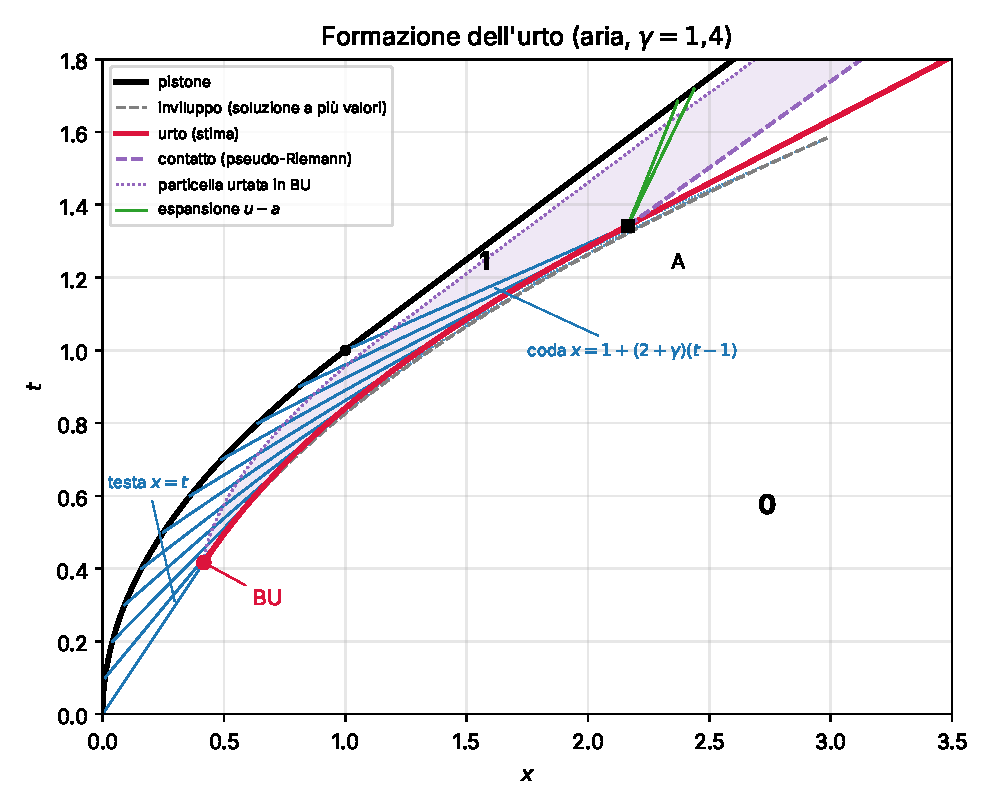
\includegraphics[width=0.78\textwidth]{xt_formazione.pdf}
  \caption{Piano $x$--$t$ fino a $t=1{,}8$ (aria): caratteristiche $\upa$ emesse dal pistone (tratto fisico
  continuo, prolungamento a più valori punteggiato fino all'inviluppo), urto stimato da BU ad A, contatto ed
  espansione $\uma$ del pseudo-Riemann. Ombreggiato il gas urtato durante la crescita dell'urto.}
  \label{fig:xtf}
\end{figure}
La fig.~\ref{fig:xtf} mostra la formazione dell'urto. Le caratteristiche si infittiscono vicino alla testa, dove
l'inviluppo (tratteggio grigio) ha il suo primo punto in BU, sulla testa stessa. Senza l'urto la soluzione sarebbe
a più valori fra la testa e l'inviluppo; l'urto taglia questa regione e assorbe una dopo l'altra le
caratteristiche, fino all'ultima, la coda uscente da $(1,1)$, raggiunta in A. La particella che l'urto investe in
BU (punteggiata) separa il gas mai urtato, una sottile striscia vicino al pistone, dal gas urtato da un urto via via
più forte.

\begin{figure}[H]
  \centering
  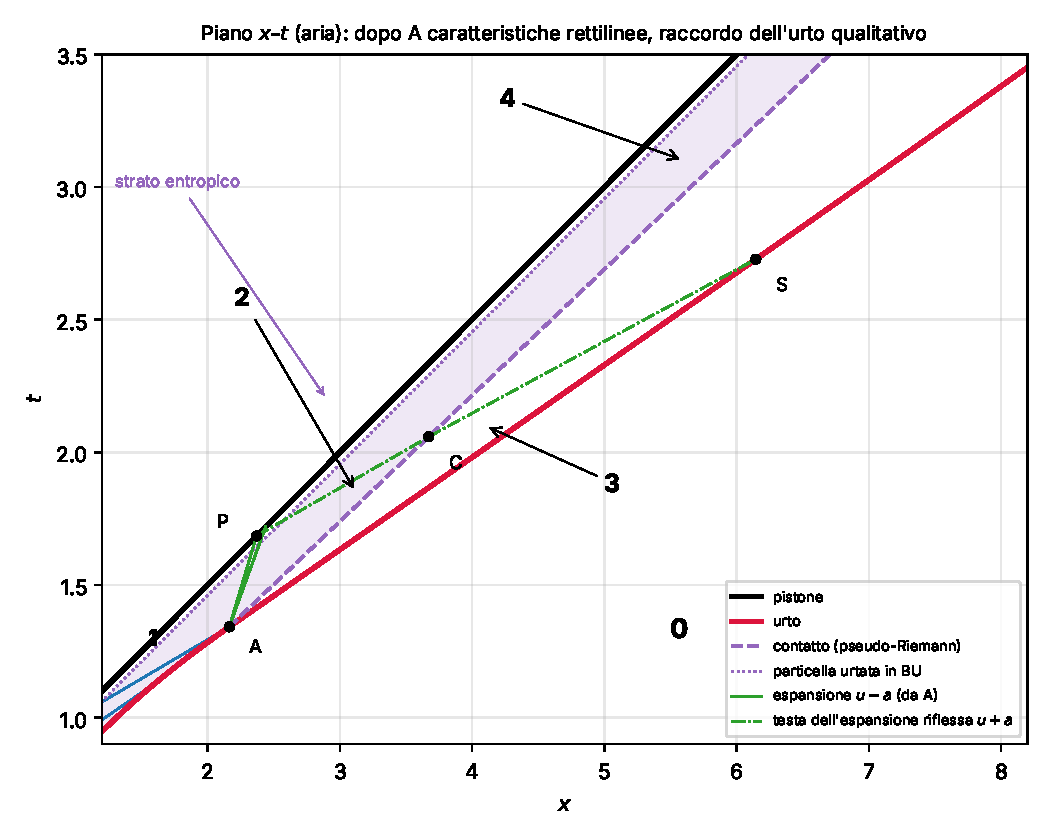
\includegraphics[width=0.8\textwidth]{xt_campo.pdf}
  \caption{Piano $x$--$t$ dopo A (aria), con caratteristiche rettilinee: espansione $\uma$ da A al pistone (P),
  testa dell'espansione riflessa $\upa$ attraverso il contatto (C) fino all'urto (S); dopo S l'urto rallenta verso
  $w_\infty$ (raccordo qualitativo).}
  \label{fig:xtc}
\end{figure}
Nella fig.~\ref{fig:xtc} pistone, contatto e urto sono rette di pendenza vicina: il pistone va a $2$, il contatto a
\num{2.11}, l'urto a \num{2.87}. Il gas 1 e il gas 2 occupano zone sottili fra pistone e contatto; l'espansione
$\uma$, pur andando verso destra nel laboratorio, viene raggiunta dal pistone in P. L'espansione riflessa attraversa
il contatto in C e raggiunge l'urto in S; da lì in poi la traiettoria dell'urto si incurva verso la pendenza
asintotica \num{2.76}, mentre fra pistone e urto si stabiliscono gli stati 5 e 6.

\begin{figure}[H]
  \centering
  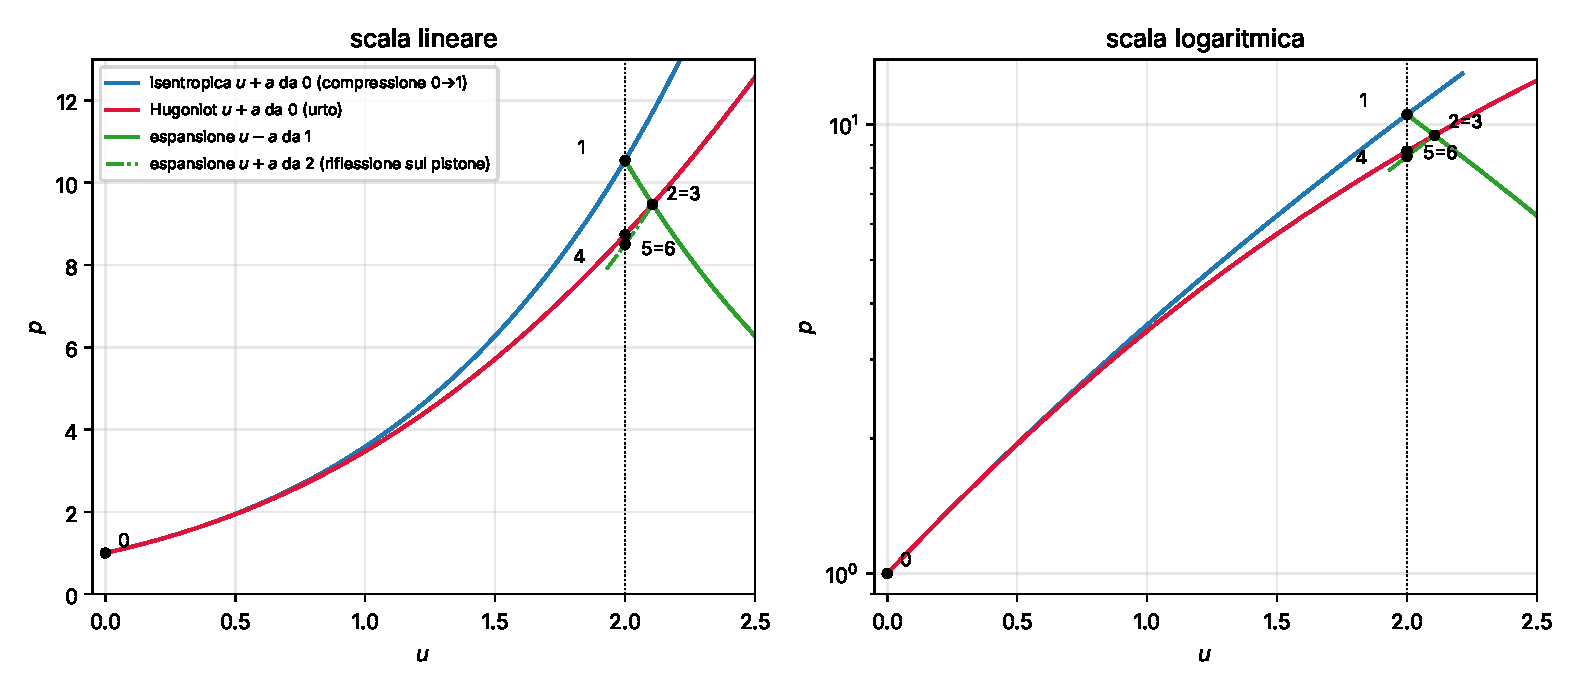
\includegraphics[width=\textwidth]{pu.pdf}
  \caption{Piano $p$--$u$ (aria), in scala lineare e logaritmica: isentropica $\upa$ e curva di Hugoniot $\upa$ da
  0, espansione $\uma$ da 1, espansione $\upa$ da 2 (riflessione sul pistone), retta $u=u_p=2$.}
  \label{fig:pu}
\end{figure}
\begin{figure}[H]
  \centering
  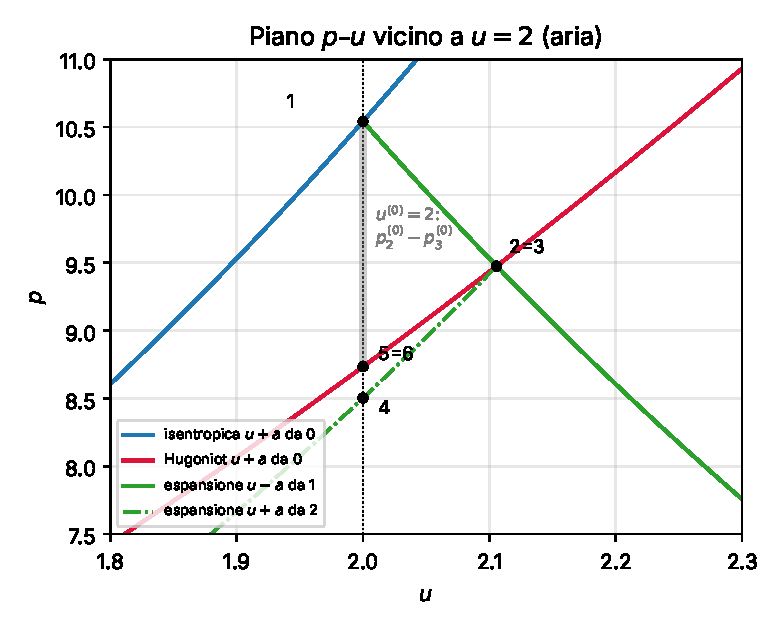
\includegraphics[width=0.62\textwidth]{pu_zoom.pdf}
  \caption{Piano $p$--$u$ vicino a $u=2$ (aria): residuo del primo tentativo isentropico ($u^{(0)}=2$) e stati del
  transitorio.}
  \label{fig:puz}
\end{figure}
Nel piano $p$--$u$ (fig.~\ref{fig:pu}) la compressione del pistone porta da 0 a 1 lungo l'isentropica $\upa$;
la curva di Hugoniot da 0 ha la stessa tangente in 0 e sta sotto l'isentropica per $u>0$: le due coincidono finché
la compressione è debole e si separano visibilmente sopra $u\approx1$. In scala lineare si leggono le distanze in
pressione fra le curve vicino a $u=2$; in scala logaritmica la curvatura è attenuata e si vede che le due curve
partono tangenti da 0. Nello zoom (fig.~\ref{fig:puz}) la retta verticale fra 1 e la Hugoniot in $u=2$ è il
residuo del primo tentativo; lo stato 2=3 è l'intersezione dell'espansione $\uma$ da 1 con la Hugoniot. Lo stato
4 sta sulla retta $u=2$, sotto la Hugoniot; il regime asintotico 5=6 sta sulla Hugoniot in $u=2$. Gli stati 5 e 6
coincidono in $p$--$u$ ma hanno impedenze diverse ($\rho_5a_5=\num{8.97}$, $\rho_6a_6=\num{7.88}$): il contatto
non si vede in questo piano.

\begin{figure}[H]
  \centering
  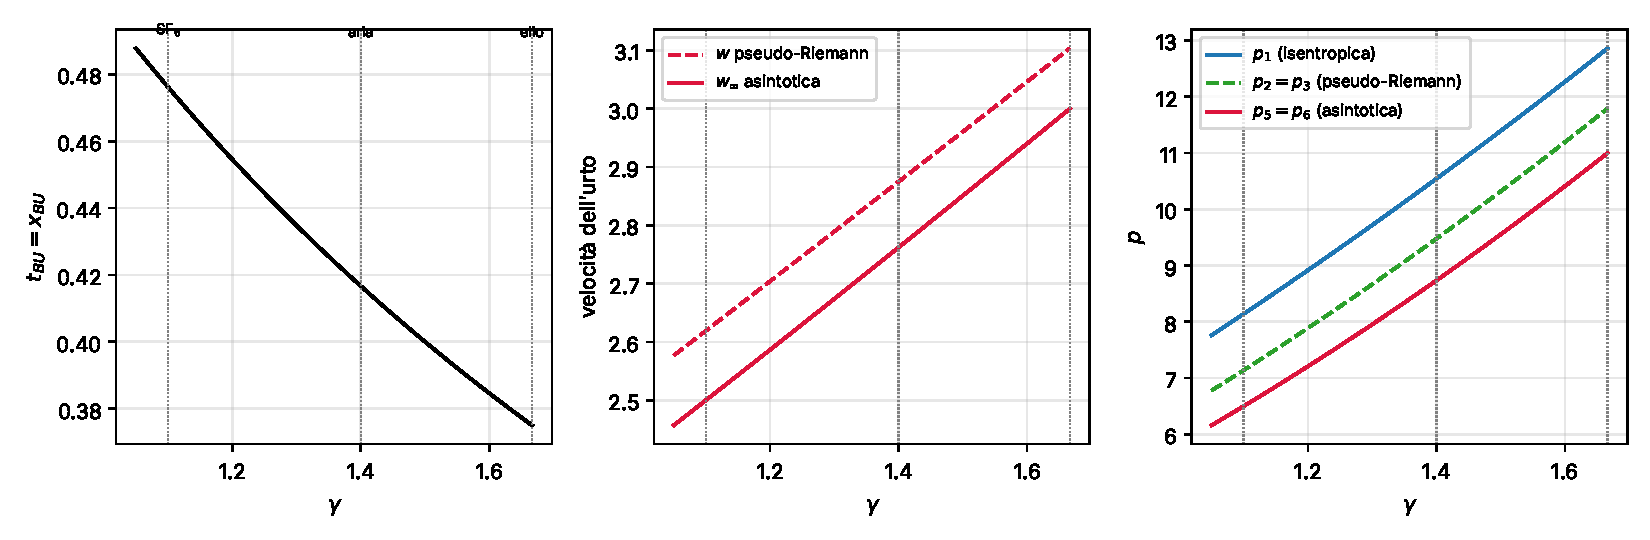
\includegraphics[width=\textwidth]{gas.pdf}
  \caption{Dipendenza da $\gamma$: istante di formazione, velocità dell'urto (pseudo-Riemann e asintotica),
  pressioni dei plateau. Le rette punteggiate indicano SF$_6$, aria ed elio.}
  \label{fig:gas}
\end{figure}
La fig.~\ref{fig:gas} riassume la dipendenza dal gas: al crescere di $\gamma$ il blow-up è più precoce, l'urto più
veloce e le pressioni più alte; la differenza fra la velocità del pseudo-Riemann e quella asintotica resta di circa
$0{,}1$--$0{,}12\,a_0$ per tutti i gas.

%==============================================================================
\section{Discussione fisica}
\textbf{Peso molecolare.} Un gas leggero monoatomico ha $\gamma$ alto, un gas pesante poliatomico $\gamma$ vicino a 1.
A pari $a_0$, con $\gamma$ alto la velocità caratteristica $u+a=a_0+(1+\delta)u$ cresce di più con $u$: la non
linearità è più forte, l'urto si forma prima ed è più veloce e la pressione è più alta (elio: $w_\infty=3$,
$p_6=11$). Con $\gamma\to1$ il gas è più comprimibile: l'urto è più lento e la pressione più bassa, ma la densità
dietro l'urto è maggiore (SF$_6$: $\rho_6/\rho_0=5$ contro 3 per l'elio) e il riscaldamento minore
($T_6/T_0=\num{1.30}$ contro \num{3.67}). $R$ cambia solo la scala delle temperature. Se invece si confrontassero
gas reali alla stessa temperatura, il dato in unità di $a_0$ nasconderebbe il peso molecolare:
$a_0=\sqrt{\gamma RT_0}$ è circa \SI{1000}{m/s} per l'elio e \SI{135}{m/s} per SF$_6$ a \SI{293}{K}, quindi la
stessa legge del pistone in m/s sarebbe una compressione debole nell'elio e fortissima in SF$_6$.

\textbf{Isentropica contro urto.} Il pistone ``comprime meglio'' di un urto: lo stato 1 raggiunto isentropicamente
ha pressione maggiore di quella che un urto può sostenere alla stessa velocità del gas. Per questo, quando l'urto
ha inglobato la compressione, nasce l'espansione $\uma$ e l'urto si trova temporaneamente più forte di quello
asintotico ($w=\num{2.87}$ contro \num{2.76}); l'espansione riflessa dal pistone lo riporta al valore del pistone
impulsivo. È lo stesso meccanismo del problema di Friedrichs, con la differenza che qui il pistone non si ferma.

\textbf{Strato entropico.} L'intensità dell'urto cresce da zero in BU fino al massimo vicino ad A e poi cala verso
il valore asintotico. Le particelle portano l'entropia ricevuta: fra il gas mai urtato vicino al pistone ($s_0$) e
il gas 6 l'entropia prima cresce fino a $\approx s_3$ e poi scende a $s_6$. Lo strato è continuo e non c'è un
vero contatto: il contatto del pseudo-Riemann lo rappresenta in modo concentrato. Nel modello il gas fra pistone e
contatto (stati 1, 2, 4) ha l'entropia iniziale; in realtà la maggior parte di quel gas è stata urtata durante la
crescita dell'urto e il gas a $s_0$ è solo una striscia sottile vicino al pistone. Gli stati 2, 3 e 4 sono quindi
indicativi, mentre il regime asintotico (urto, stato 6 e pressione) è esatto: dipende solo dalla velocità del
pistone. Allo stesso modo gli istanti P, C, S sono stime, perché le caratteristiche nelle zone d'interazione sono
curve.

\textbf{Pressione sul pistone.} Cresce isentropicamente, $p_p=(1+2\delta t)^{2\gamma/(\gamma-1)}$, fino a
$p_1=\num{10.5}$ in $t=1$, resta costante finché non arrivano le onde riflesse dall'urto (nel modello
l'espansione da A, in $t\approx\num{1.7}$), scende a $\approx\num{8.5}$ e risale lentamente verso \num{8.73} per le
deboli compressioni riflesse dal contatto.

\textbf{Limiti del modello.} Il modello 1D non viscoso trascura lo strato limite e lo scambio termico con le pareti;
con $T_6/T_0\approx\num{2.4}$ per l'aria a temperatura ambiente si arriva a circa \SI{700}{K}, dove il gas perfetto
caloricamente è ancora ragionevole.

\end{document}
